\chapter{Development Practices} %remember to say how we work with costumers
\label{sec:developmentpractice}
\myTop{An important part of this project is the collaboration between the peer-groups, which is guided through a development method. 
This chapter gives a description of how we are using the development method \sos{} in our sub-group, and which additional practices we have chosen to use.}%
We distinguish between a development method and a development practice.
A development method is a collection of development practices that in combination should enhance development in general. 
A development practice is a predefined set of actions that are performed during development.



\section{Utilizing the Development Method}
%utilizing agile methods -> we don't know shit so its good
Since we are not familiar with Moodle from the beginning of the project, we do not have a full understanding of how the entire system should be structured and created.
We solve this problem by using the development method \scrum{} and dividing the development process into a number of sprints.
%Ideally after each sprint we should have a fully functional system, which is in such a state that it can be shipped.
%This is not entirely the case, since we need a lot of information before we can start programming.
%We do not aim to have a functional system after each sprint, due to the fact that we are developing a new system based on an unfamiliar platform and we have short sprints. 

%sprints

Our first sprint consists of information gathering; we study the Moodle platform as well as interview our end users in order to get a few initial requirements. 
We plan this non-programming sprint to learn and experience the \scrum{} development method before we start a programming sprint.
%in spite of  \scrum{} being intended for development. 

Different sources suggest different notations for what is in a backlog~\cite[p.~17]{scrumchecklist}\cite[pp.~123-124]{Larman04}.
Our backlog items are all features. 
See \figref{fig:backlog} that illustrates the relation between the backlogs. 
\begin{figure}%
\center
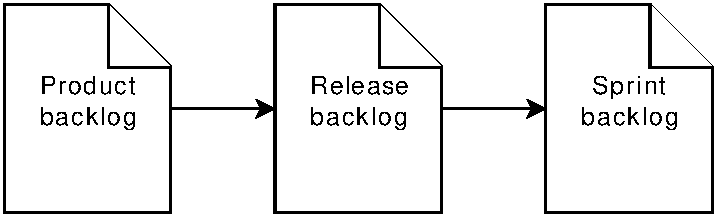
\includegraphics[scale=0.50]{images/backlogs}%
\morscaption{Illustration of how backlog items move through the different backlogs}%
\label{fig:backlog}%
\end{figure}

%product backlog
The requirements we gather are used to create feature descriptions, which are used to fill the product backlog.
%sprint backlog
At the beginning of each succeeding sprint we choose items from the product backlog and move them to the sprint backlog, which is a list of features we expect to implement in the particular sprint.

Before an item is moved to a sprint backlog it is moved to the release backlog.
This means that the release backlog consists of all items implemented in the sprints of this semester.


%planning poker
In order to choose which items to move to the sprint backlog we assign each item currently in the product backlog a number of story points.
We do this by playing planning poker, which is a card game where we all give our estimates of the items on the backlog simultaneously. 
If there is a significant difference between the estimates we discuss the scope of the feature and argue until an agreeable estimate is found.
Additionally, we assign the items a priority.
Based on the estimate and priority we choose which items we are able to implement in the current sprint.

%burndown chart
As we progress in the sprint the number of remaining story points starts to dwindle. 
We keep track of this by a burndown chart, which is a physical chart with a line that shows the expected progress.
The total number of remaining story points is plotted on the graph each day, so we can see if we are progressing at a satisfactory rate.

\begin{comment}
%daily scrum
In our sub-group we start each day with a \scrum{} meeting.
In this short meeting we all stand up and each tell three things: What we did since last \scrum{} meeting, what we are going to do today, and which -- if any -- impediments we have.
This gives the entire group an idea of what is being worked on, and by doing this everybody always have a task they have chosen themselves.
\end{comment}



\section{Inter Group Development Method}
Since all sub-groups depend on each other in the multi-project, we need to organize what each sub-group is doing.
%We do this in two ways: in between sprints and during sprints.

%sprint planning meetings

At the sprint planning meeting at the beginning of each sprint all the sub-groups present their plan for what they are going to produce in the coming sprint.
If other sub-groups have any dependencies, they communicate these, and the sub-groups collaboratively decide the overall tasks each sub-group should accomplish in the given sprint.

%demo meetings
At the end of each sprint the sub-groups meet and present what they have created during the sprint.
%Depending on the state of the system end-users can be invited to these meetings.
%End users can be invited to be showcased specific aspects of the system by individual sub-groups in order to acquire feedback between sprint.
End users can be invited to be showcased or try the system in demo meetings in order to acquire feedback between sprints.


%weekly casual scrum og scrum meetings
During sprints the sub-groups work together to some extent.
Since we all work close to each other we can always go to each others physical group room to ask for help or request that some specific work should be done.
Additionally we hold \sos{} meetings approximately twice a week.
In these meetings the \scrummaster{}s of all the sub-groups meet and discuss the direction of the project and share information regarding how the sub-systems should be integrated with the different components that the sub-groups are developing.


\section{Additional Practices}
Since we are continuously integrating -- a \scrum{} practice -- and are passing the project on to new developers next year (described in item 5 in \secref{subsec:choosingmethod}), we want automated tests that can be run to ensure no regression in functionality. 
We have already decided that we are using the built-in test framework of \moodle{} in \secref{sub:testing}.
To make sure that test cases are written and to avoid that these are created in the last minute we use test driven development (TDD)~\cite[pp.~292-294]{Larman04} as an additional development practice.
TDD states that test cases must be written before the functionality to be tested is written.
A functionality is not considered implemented until the test case(s) for it are written and pass.
These test cases can be run whenever a change is made to existing code to test whether the change broke something.
